\subsection{Analyzing Data}
\subsubsection{Displaying Data}
If we have the table:\\

\begin{tabular}{c|c|c|c|c}
    Drink & Type & Calories & Sugar (g) & Caffeine (mg)\\
    \hline
    coffee & hot & 4 & 0 & 260\\
    latte & hot & 100 & 14 & 75\\
    mocha & hot & 170 & 27 & 95
\end{tabular}\\
The \textit{individuals} are defined to be the drinks in this case (the things we are collecting data from).\\
There are also 4 variables. The variable "Type" is \textit{categorical}, meaning that the data it holds fits into one of some number of categories (digital vs. analog).\\
Some types of graphs we can use to represent data includes pictographs, bar graphs, frequency graphs, pie graphs, and many more.\\
Ex: Bar graph\\
\centerline{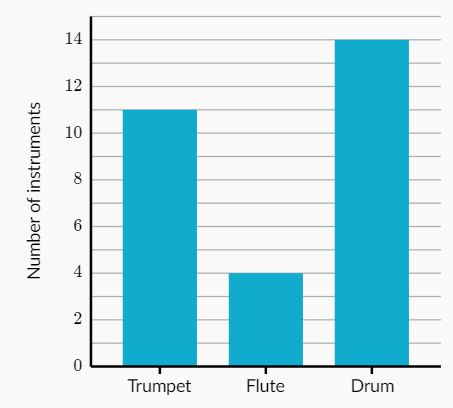
\includegraphics[scale=0.7]{Images/FundamentalsPictures/barGraph.png}}
Data that relates to itself, we can represent with a two-way table.\\
Ex: Say we have 10 candies, 6 chocolate, 3 chocolate-coconut, 1 coconut, and 2 plain. We can express this as\\
\begin{tabular}{c|c|c}
    & Coconut & No Coconut\\
    \hline
    Chocolate & 3 & 6\\
    No Chocolate & 1 & 2
\end{tabular}\\
A two-way table with relative frequencies is when the columns are normalized to equal 1.\\
\begin{tabular}{c|c|c}
    & Coconut & No Coconut\\
    \hline
    Chocolate & 75\% & 75\%\\
    No Chocolate & 25\% & 25\%
\end{tabular}\\
\textit{Conditional distribution} is when you analyze a single row/column or a subset of the table.\\
\textit{Marginal distribution} is when you analyze the totals of the rows/columns.\\
Frequency plots are similar to bar graphs but are more all-encompassing. We can use frequency graphs to represent data that is more analog than discrete, called a histogram.\\
Ex:\\
\centerline{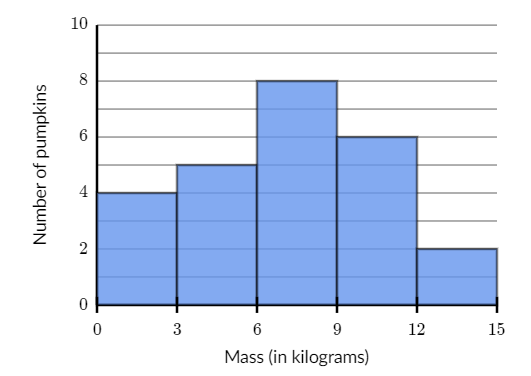
\includegraphics[scale=0.7]{Images/FundamentalsPictures/histogram.png}}
With histograms we can classify different behaviors of the data.\\
The maximum value of the histogram is the \textit{peak}.\\
If there are groupings of data points in a similar area, we call those \textit{clusters}\\
If there are a small number of data points far away from the majority of the data, we call those \textit{outliers}.\\
We can also represent frequency data using a stem-leaf plot.\\
Ex:\\
\begin{tabular}{c|l}
    Stem & Leaf\\
    \hline
    0 & 0, 0, 2, 4, 7, 7, 9\\
    1 & 1, 1, 3, 8\\
    2 & 0
\end{tabular}\\
maps to the data 0, 0, 2, 4, 7, 7, 9, 11, 11, 13, 18, 20.\\
The stem maps the tens place value and the leaf maps the ones place value

\subsubsection{Center and Spread}
The average of a set of data is a measure of central tendency of that data and there are many ways to express the average.\\
The \textit{mean} is the arithmetic sum of the data divided by the number of data points
$$\mu=\frac{1}{N}\sum_{i=1}^N x_i$$
The \textit{median} is the middle value of the data set. If there are an even number of data points, the median is the mean of the two middle data points.\\
The \textit{mode} is the most commonly occurring value.\\
The \textit{midrange} is the mean of the difference between the maximum and minimum values in the data set.\\

Mean is the standard measure for average in most cases, though it is important to note that outliers can sometimes have a large, unwanted, effect on the mean so in these cases, it may be best to use median as the average.\\

Data sets can have the same averages but may look very different. To represent this, we introduce spread. Spread is how spread out the data points are.\\
The most simple measure of spread is the \textit{range} which is simply the difference between the maximum and minimum values in the data set.\\
A slightly more elaborate method of calculating spread is the \textit{mean absolute deviation} (MAD). This is the mean of how far away a number is from the mean.
$$MAD=\frac{1}{N}\sum_{i=1}^N|x_i-\mu|$$
The \textit{interquartile range} (IQR) is analogous to the median of a data set. The IQR is the difference between the 1st and 3rd quartiles in a data set. The first quartile is the median of the lower half of the data and the 3rd quartile is the median of the higher half of the data.\\
Ex: For data of 1,3,3,3,4,4,4,6,6,\\
Median$=4$\\
$Q_1=\text{median}\brcurly{1,3,3,3}=3$\\
$Q_3=\text{median}\brcurly{4,4,6,6}=5$\\
IQR$=5-3=2$\\
We can use the IQR to represent data as a box and whisker plot:\\
\centerline{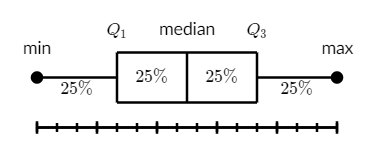
\includegraphics[scale=1]{Images/FundamentalsPictures/boxPlot.png}}\\
We can also use the IQR to define outliers. We can use the general rule of 1.5 times the IQR. Any outliers can be defined to be less than $Q_1-1.5\cdot IQR$ or greater than $Q_3+1.5\cdot IQR$\\
\textit{Variance} is the mean of the squared distance between the value and the mean, represented by $\sigma^2$
$$\sigma^2=\frac{1}{N}\sum_{i=1}^N (x_i-\mu)^2$$
By expanding the quadratic and using the definition of the mean, we can also write this as
$$\sigma^2=\frac{1}{N}\sum_{i=1}^N x_i-\mu^2$$
The \textit{standard deviation} is the square root of the variance.
$$\sigma=\sqrt{\frac{1}{N}\sum_{i=1}^N (x_i-\mu)^2}$$
We can use the standard deviation to calculate Z-scores. A Z-score is how many standard deviations a data point is from the mean.
$$Z_i=\frac{x_i-\mu}{\sigma}$$
In an ordered list of data, we can calculate the percentile by dividing the position of the data point by the number of data points in the sample size. Note that the median corresponds to the 50th percentile. Z-scores are particularly useful in calculating percentiles as we can use the aid of Z-tables to compute percentiles along a normal distribution.
